\subsection{License}

The choice upon license choice was concluded with the election of GNU General Public License v3.0 for both front- and backend applications.

First, the dependencies were collected along with their licenses into json files by using NPM License Checker and  a .NET utility tool~\cite{NPMLicenseChecker}~\cite{nugetLicense}.

Results can be created by the following commands respectively:

\begin{itemize}[noitemsep]
    \item 
\begin{verbatim}
license-checker --json --out `<path-of-output-file>`
\end{verbatim}

    \item 
\begin{verbatim}
dotnet-project-licenses -i `<path-of-project>` -u -o -j
\end{verbatim}

\end{itemize}

Regarding the frontend, only one dependency seemed alarming at first glance, which was the \texttt{node-forge} package~\cite{nodeForge}. Its license is BSD-3-Clause OR GPL-2.0. SonarAnalyzer. CSharp was concerning on the backend side as it has LGPL-3.0-only license~\cite{sonarlint}. Both of these discoveries contained a form of a protective license, hence the caution on our side. However, the source code does not contain derivative work of the library. It is designed to work with it, so it falls outside the scope of the protective licenses.
\vspace{3mm}

Additionally, we have used ScanCode-toolkit to scan the two projects~\cite{scanCodeToolkit}. The results were parsed into json files that could be fed into ScanCode-Workbench - a visual application detailing the contained licenses, copyrights with different charts and diagrams~\cite{scanCodeWorkbench}.

\begin{figure}[h]
    \centering
    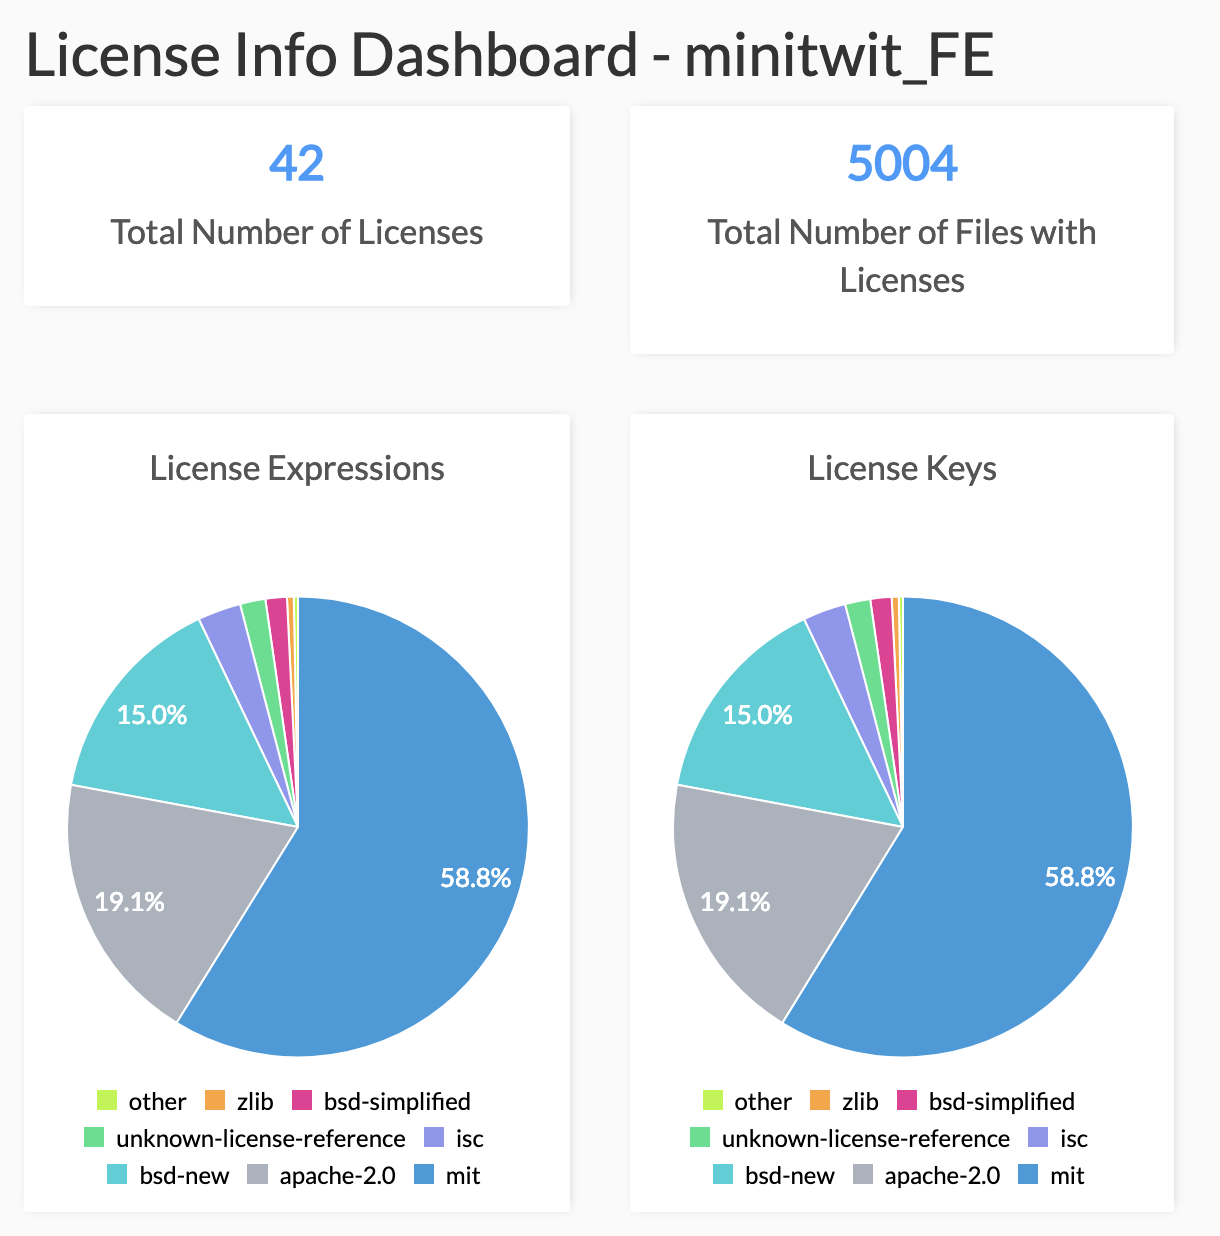
\includegraphics[width=0.5\textwidth]{images/license/scancode_workbench_fe_results.png}
    \caption{ScanCode Workbench Dashboard}
    \label{fig:license}
\end{figure}

JSON files can be generated by the command below, assuming ScanCode-Toolkit is installed: \\

\begin{verbatim}
`<path-to-scancode | ./scancode on Windows>` -clpeui -n 2 --json-pp 
<output-json-file-name> <project-to-be-scanned-directory>`
\end{verbatim}

\vspace{3mm}

Eventually, we wanted our software to have:

\begin{itemize}[noitemsep]
    \item the freedom to use it for any purpose,
    \item the freedom to change it to suit needs,
    \item the freedom to share it
    \item the freedom to share the changes made
\end{itemize}

By using GPL v3, we make sure that this freedom is also protected in derivative works as well. Additionally, it includes an explicit grant of patent rights, which protects against potential patent trolling.

\subsubsection*{Future considerations}
Future considerations include using ScanCode.io and ScanPipe~\cite{scanCodeIO}~\cite{ScanPipe}. By providing a \texttt{policies.yml} file in the root folder we can define our own license policies and compliance alerts. The scan result of a json file would include if there is a risk in using a particular dependency. Another solution is to further utilize what is already in the pipeline, which is the docker scanning tool provided by Snyk~\cite{snyk}. Unfortunately, scanning for licenses are only part of their business plan. Defining our own license policies will include alerts of different levels with optional instructions intended for developers of steps that should be taken to negate the compliance issues. License results could be handled in our existing script dockerScanner.bash~\cite{dockerScanner}.